\documentclass[journal,onecolumn]{IEEEtran}
\usepackage{amsmath,amssymb,graphicx,booktabs,multirow,array,longtable,url}
\usepackage[hidelinks]{hyperref}
\newcommand{\cb}{\texttt{cost\_bid}}
\newcommand{\gb}{\texttt{group\_bid}}
\renewcommand{\thesection}{S-\Roman{section}}
\renewcommand{\thetable}{S-\Roman{table}}
\renewcommand{\thefigure}{S\arabic{figure}}
\begin{document}
\title{Supplementary Material for ``Who Backs Up? Benchmarking Decentralized Multi-Robot Yield Negotiation in Narrow Corridors''}
\author{Roshan George, Martin Glavin, Edward Jones, and Brian Deegan}
\maketitle
Equation, table, and section numbers without the prefix S refer to the main paper.

\section{Notation and Parameters}
\begin{table}[!ht]\centering
\caption{Summary of Principal Mathematical Notation.}
\label{tab:nomenclature}
{\footnotesize\renewcommand{\arraystretch}{1.28}\setlength{\tabcolsep}{3.5pt}\medmuskip=2mu\thickmuskip=3mu
\resizebox{0.7\columnwidth}{!}{\begin{tabular}{@{}ll@{}}\toprule
Symbol & Definition \\\midrule
\multicolumn{2}{@{}l}{\emph{Sets, Indices, and Refuges}} \\\addlinespace[2pt]
$i \in \{A, B\}$; $Y, P$ & Robot index; candidate yielder and proceeder \\
$\mathcal{G}_Y, \mathcal{G}_P$ & Yielding and proceeding convoy robot groups \\
$\mathcal{R},\, r \in \mathcal{R}$ & Discrete refuge set and individual refuge index \\
$x_r, w_r, y_{\mathrm{park},r}$ & Refuge entry coordinate, width, and parking offset \\
$\mathcal{F}(Y,P),\, r^\ast$ & Feasible refuge set for $(Y,P)$ and delay-optimal refuge \\\addlinespace[2pt]\midrule
\multicolumn{2}{@{}l}{\emph{Robot State and Feasibility (Eqs.~(1)--(3))}} \\\addlinespace[2pt]
$x_i, v_i, s_i \in \{\pm 1\}$ & Longitudinal position, speed, and travel direction \\
$x_{\mathrm{goal},i}, t_{\mathrm{enter},i}$ & Goal coordinate and corridor entry timestamp \\
$u_i \ge 1,\, l_i \in \{0,1\}$ & Task urgency weight and binary payload flag \\
$v_{\max,i}, v_{\mathrm{rev},i}, v_Y^{\mathrm{app}}$ & Forward, reverse, and refuge-approach speed limits \\
$x_{\mathrm{stop}}, x_{\mathrm{hold}}, x_{\mathrm{pass}}$ & Proceeder braking, hold, and refuge-clearance lines \\\addlinespace[2pt]\midrule
\multicolumn{2}{@{}l}{\emph{Maneuver Timeline and Delay (Eqs.~(4)--(6))}} \\\addlinespace[2pt]
$T_i^{\mathrm{free}}, t_{\mathrm{turn}}$ & Free-flow travel time and $90^\circ$ bay-turn duration \\
$t_{\mathrm{park}}, t_{\mathrm{hold}}, t_{\mathrm{go}}, t_{\mathrm{pass}}$ & Park, hold-arrival, proceeder-release, and clearance times \\
$T_i(r),\, d_i(r)$ & Total arrival time and encounter delay via refuge $r$ \\
$C_{\mathrm{soc}}(Y,r)$ & Pairwise urgency-weighted social delay cost \\\addlinespace[2pt]\midrule
\multicolumn{2}{@{}l}{\emph{Bidding, Incentives, and Evaluation (Eqs.~(7)--(12))}} \\\addlinespace[2pt]
$\tilde{c}_Y,\, \sigma,\, \epsilon_Y$ & Noisy social-cost bid, log-normal noise scale, and draw \\
$C_{\mathrm{grp}}(\mathcal{G}_Y,\mathcal{G}_P)$ & Side-level convoy group-bidding social cost \\
$o \in \{A,B\},\, o^\ast$ & Candidate yield outcome and mechanism-selected outcome \\
$b_i(o),\, p_i$ & Reported delay cost for outcome $o$ and Clarke VCG payment \\
$D_{i,t}^{\mathrm{cum}},\, \lambda$ & Cumulative delay through encounter $t$ and fairness weight \\
$D_\pi^{(k)},\, \Delta_\pi$ & Episode delay on encounter $k$ and paired excess delay \\\bottomrule
\end{tabular}}}
\end{table}

\begin{table}[!ht]
\caption{Default physical, kinematic, and protocol parameters calibrated to the ROBOTIS TurtleBot3 Waffle~\cite{turtlebot3}.}
\label{tab:params}
\centering
{\footnotesize\setlength{\tabcolsep}{2.5pt}\medmuskip=2mu\thickmuskip=3mu
\resizebox{0.7\columnwidth}{!}{\begin{tabular}{@{}lr@{}}\toprule
Parameter (Symbol) & Default Value \\\midrule
\multicolumn{2}{@{}l}{\emph{Geometry}} \\
Corridor dimensions ($L \times W$) & $8.0$ (or $10.0$)\,m $\times 0.65$\,m \\
End-room dimensions & $2.5 \times 2.5$\,m ($y_{\mathrm{park}} = \pm 0.90$\,m) \\
Pull-in bay dimensions ($w_b \times d_b$) & $0.80 \times 0.60$\,m ($y_{\mathrm{park}} = \pm 0.625$\,m) \\
Required wall/peer clearance ($c_{\mathrm{clear}}$) & $0.05$\,m \\\midrule
\multicolumn{2}{@{}l}{\emph{Waffle Kinematics}} \\
Chassis footprint ($l_{\mathrm{rob}} \times w_{\mathrm{rob}}$) & $0.281 \times 0.306$\,m \\
Rotational swept radius ($R_{\mathrm{sw}}$) & $0.25$\,m \\
Forward / reverse speed ($v_{\max} / v_{\mathrm{rev}}$) & $0.26$\,m/s / $0.15$\,m/s \\
Max turn rate ($\omega_{\max}$) & $1.82$\,rad/s \\
Linear / angular accel.\ ($a_{\max} / \alpha_{\max}$) & $0.5$\,m/s$^2$ / $3.0$\,rad/s$^2$ \\\midrule
\multicolumn{2}{@{}l}{\emph{Sensing \& Communication}} \\
Control loop / \texttt{STATE} / \texttt{BID} rate & $20$\,Hz / $5$\,Hz / $3.3$\,Hz ($0.3$\,s) \\
Radio conflict / Lidar range ($R_{\mathrm{det}} / R_{\mathrm{Lidar}}$) & $6.0$\,m / $3.5$\,m \\
Nominal latency ($\tau$) + jitter ($j$) & $0.05$\,s + $U[0, 0.02]$\,s \\
State freshness / neg.\ timeout ($\tau_{\mathrm{state}} / \tau_{\mathrm{neg}}$) & $1.0$\,s / $3.0$\,s \\
Episode horizon ($T_{\max}$) & $180.0$\,s \\\bottomrule
\end{tabular}}}
\end{table}

\section{Extended RQ1 Results}
\subsection{Original bid-noise grid}
Fig.~\ref{fig:rq1_noise} shows the original five-point \texttt{S7} grid (1,470 unique episodes; the released file stores 3,150 rows because the $\sigma$-independent runs repeat for each $\sigma$). The densified and heterogeneous grids are in Table~IV of the main paper.
\begin{figure}[!ht]\centering
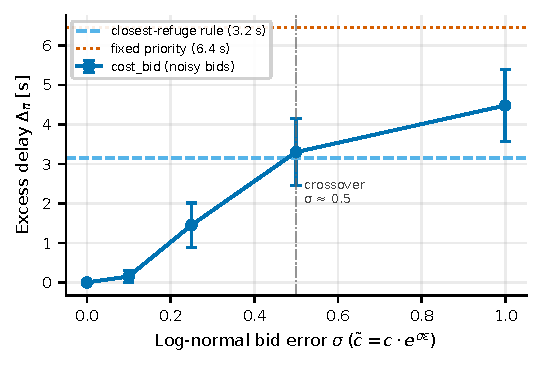
\includegraphics[width=\columnwidth]{Images/fig7_bid_noise.pdf}
\caption{Sensitivity of \cb\ excess delay $\Delta_\pi$ to multiplicative log-normal bid estimation error $\sigma$ (\texttt{S7}, 1,470 unique episodes; dashed lines: \texttt{rules\_proximity} on the same \texttt{S7} draws and \texttt{fixed\_priority} on the \texttt{S1} draws). Error bars show 95\% CIs.}
\label{fig:rq1_noise}
\end{figure}

\subsection{Tabular outcome classifier}
The classifier (\texttt{learned}) keys each conflict on binned distances to the nearest feasible refuge behind each robot, the sign of $u_A-u_B$, and both payload flags. It is trained on two-bay encounters by simulating both forced outcomes, so every training encounter reveals the delay of both actions (full information). Training sizes of 50, 200, and 800 encounters give held-out two-bay excess delays $\Delta^{w}$ of $+3.9\pm1.7$, $+2.8\pm1.5$, and $+2.6\pm1.1$\,s (150 episodes each; \texttt{rules\_default} $+2.5\pm1.0$\,s), with $35\%$, $8\%$, and $0.7\%$ of encounters falling back to \texttt{fixed\_priority} on unseen keys. On the unseen single-bay layout the three sizes give $+13.6\pm3.4$, $+14.7\pm3.5$, and $+13.1\pm4.1$\,s, so more training data does not close the generalization gap. At 800 encounters, the 128 seen-key single-bay encounters average $+13.6\pm4.6$\,s and the 22 unseen-key encounters $+10.5\pm6.8$\,s.
\begin{figure}[!ht]\centering
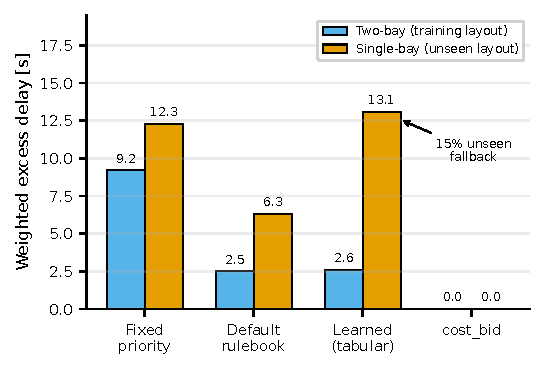
\includegraphics[width=\columnwidth]{Images/fig8_bandit_generalization.pdf}
\caption{Tabular outcome classifier (\texttt{learned}) weighted excess delay on its training two-bay layout versus an unseen single-bay layout ($150$ evaluation episodes per layout).}
\label{fig:rq1_bandit}
\end{figure}

\section{Extended RQ3 Results}
\subsection{Safeguard ablation}
\begin{table}[!ht]\centering
\caption{Factorial safeguard ablation (\texttt{S8c}) under 90--99\% packet loss and 2--8\,s latency ($v_{\max}=0.5$\,m/s; 360 episodes per row; \texttt{bay\_check} had zero triggers and identical metrics, so its 8 duplicate rows are condensed). Collisions were 0 in every arm (95\% upper bound 1.06\%).}
\label{tab:abl}
{\footnotesize\setlength{\tabcolsep}{3.4pt}
\begin{tabular}{@{}lccrrrr@{}}\toprule
Policy & \texttt{commit} & \texttt{state} & Succ.\ [\%] & Deadl. & Delay [s] & Dual [\%] \\\midrule
\multirow{4}{*}{\texttt{fixed\_pr.}}
 & \checkmark & \checkmark & 99.2 & 3 & $89.8\pm3.9$ & 21.9 \\
 & \checkmark & --         & 99.2 & 3 & $90.0\pm4.0$ & 23.6 \\
 & --         & \checkmark & 98.1 & 7 & $86.0\pm3.6$ & 15.3 \\
 & --         & --         & 98.6 & 5 & $86.8\pm3.7$ & 16.4 \\\midrule
\multirow{4}{*}{\cb}
 & \checkmark & \checkmark & 98.9 & 4 & $79.6\pm3.9$ & 17.8 \\
 & \checkmark & --         & 99.2 & 3 & $79.9\pm3.9$ & 18.6 \\
 & --         & \checkmark & 99.4 & 2 & $76.4\pm3.7$ & 14.2 \\
 & --         & --         & 99.7 & 1 & $76.8\pm3.7$ & 14.7 \\\bottomrule
\end{tabular}}\\[2pt]
{\footnotesize \texttt{state}: \texttt{state\_guard}. Dual: \% of episodes where both robots entered \texttt{YIELD} before one aborted/exited.}
\end{table}

Table~\ref{tab:abl} lists all arms of \texttt{S8c}. Rows with \texttt{bay\_check} on and off produced identical episodes, so they are merged.

\subsection{Map discovery}
When robots instead discover pull-in bays as they drive in \texttt{explore} mode (1,440 base episodes plus 360 hold-mode episodes in 2D, Fig.~\ref{fig:rq3_maps}), they start knowing only the end rooms and add each bay to their map once it comes within the $3.5$\,m Lidar range. At the default radio conflict-detection range of $R_{\mathrm{det}}=6.0$\,m, waiting to share discovered bays until the robots physically detect each other on Lidar (\texttt{share\_on\_detect}) fails completely. Because the robots freeze their snapshots and make a yield decision at $6.0$\,m apart, well before their $3.5$\,m Lidar ranges ever overlap ($0/30$ maps shared in time), \texttt{share\_on\_detect} suffers the exact same delay penalty as never sharing maps at all ($+29.2$\,s for \texttt{fixed\_priority} and the rulebooks, and $+8.8$\,s for \cb). In the 2D simulator, two workarounds recover full-map refuge choices ($-0.5$\,s to $+0.1$\,s extra delay compared with knowing the full map upfront). One option is shortening the radio conflict range $R_{\mathrm{det}}$ to $3.5$\,m to match the Lidar range, and the other is enabling \texttt{hold\_for\_map}, which keeps the robots driving forward undecided for $4.9$\,s to $5.5$\,s until they detect each other on Lidar and exchange maps. Even so, simply including known bays in every \texttt{BID} message (\texttt{share\_map}) achieves $+0.0$\,s extra delay right away at $6.0$\,m without holding up the decision.
\begin{figure}[!ht]\centering
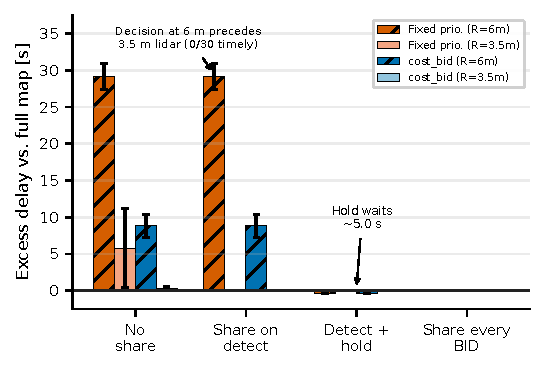
\includegraphics[width=\columnwidth]{Images/fig12_map_discovery.pdf}
\caption{Two-bay excess delay relative to full map knowledge in 2D \texttt{explore} mode ($0\%$ loss), showing why \texttt{share\_on\_detect} fails when radio negotiation ($R_{\mathrm{det}}=6$\,m) precedes $3.5$\,m Lidar range. Error bars show 95\% CIs.}
\label{fig:rq3_maps}
\end{figure}

\section{Extended RQ4 and Gazebo Results}
\begin{figure}[!ht]\centering
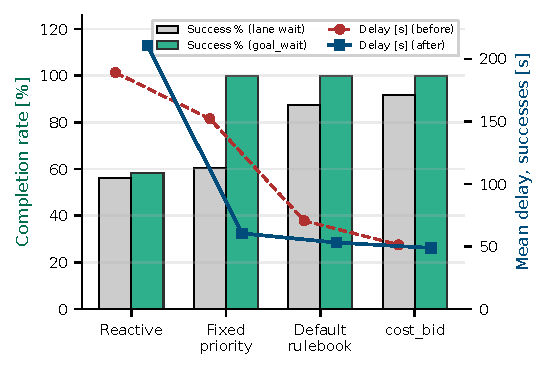
\includegraphics[width=\columnwidth]{Images/fig14_tjunction_goalwait.pdf}
\caption{Three-robot T-junction turn-in completion rate (bars, left axis) and successful-episode delay (lines, right axis) at $0\%$ loss ($n=48$ per policy) before versus after adding upstream bay waiting (\texttt{goal\_wait}).}
\label{fig:rq4_tjunction}
\end{figure}

\subsection{Gazebo limits}
Gazebo revealed three physical and perceptual limits invisible in the 2D simulator.
\begin{enumerate}
\item \emph{Lidar peer-detection lag (\texttt{explore} and \texttt{hold\_for\_map}).} Whereas \texttt{sim2d} detects an oncoming robot immediately at $3.4$\,m inside the $3.5$\,m Lidar radius, Gazebo's wall-filtered \texttt{LaserScan} clustering ($0.35$\,m cluster distance matched within $2R_{\mathrm{sw}}=0.50$\,m of peer \texttt{STATE}) only registers an oncoming Waffle at $2.3$--$2.6$\,m separation on average. Consequently, even at $R_{\mathrm{det}}=3.5$\,m, \texttt{share\_on\_detect} delivered $0/6$ maps before decision time in Gazebo versus $6/6$ in 2D (Fig.~\ref{fig:rq4_gz_trace}), adding $+7.0$\,s of mean delay to \texttt{fixed\_priority} over the full-map Gazebo baseline ($+6.8$\,s over 2D). This mean is driven by a single run: on Seed~3, Robot~$B$ was sent to \texttt{room\_hi} ($+41.7$\,s), whereas in the other five runs the robots still chose \texttt{bay1} and Gazebo delay stayed within $0.2$\,s of the full-map baseline. Enabling \texttt{hold\_for\_map} (24 Gazebo runs: 6 seeds $\times$ 2 policies $\times R_{\mathrm{det}}\in\{3.5,6.0\}$\,m) recovered the closer refuge (\texttt{bay1}) in $24/24$ runs, but peer detection occurred even closer ($1.10$--$1.18$\,m, waiting $4.7$\,s at $3.5$\,m and $9.5$\,s at $6.0$\,m), adding $+10.0$--$10.1$\,s over the full-map baseline. By then, Robot~$A$ (24/24 hold runs, $6/6$ in each policy $\times R_{\mathrm{det}}$ cell) and Robot~$B$ (20/24, $5/6$ per cell; the other four received the second bay by message) had already driven close enough to sense both bays directly, so holding worked in 3D by delaying the decision rather than by sharing maps. Including known bays in every \texttt{BID} (\texttt{share\_map}) avoids this lag entirely.
\item \emph{Branch-wall Lidar occlusion.} Early Gazebo T-junction runs showed that the $2.0$\,m side-branch walls block a parked branch robot's Lidar view of the main aisle (and exposed missing wall checks on room goals in 2D). Fusing fresh \texttt{STATE} positions into lane-clearance checks resolved this issue, meaning the final T-junction Gazebo runs serve as a post-fix verification rather than a blind transfer test.
\item \emph{Three-robot T-junction timing sensitivity ($\Delta D=-16.8$\,s).} Across all 36 T-junction runs, Gazebo accumulated $605.3$\,s less total delay than 2D ($-260.0$\,s across 18 exit runs and $-345.4$\,s across 18 turn-in runs). Event logs trace the exit gap (\cb\ $-264.7$\,s, \texttt{fixed\_priority} $+18.6$\,s, rulebook $-14.0$\,s) to a $\sim 20$\,s release-timing race. Under \cb\ in Gazebo, branch Robot~$S$ exits \texttt{bay1} slightly earlier while Robot~$A$ is still parked and slips past without triggering the second head-on conflict (or occasional $60$\,s proceed-timeout stall) seen in 2D, whereas under \texttt{fixed\_priority} and the rulebook, $S$ meets $A$ waiting in-lane and yields a second time ($4/4$ and $3/4$ runs). The larger turn-in offset ($9.5$--$28.9$\,s less delay per run and $0.4$--$6.4$\,s shorter makespan) remains an unexplained sim-to-3D timing gap, so exact T-junction delays cannot be predicted from 2D simulation alone.
\end{enumerate}
\begin{figure}[!ht]\centering
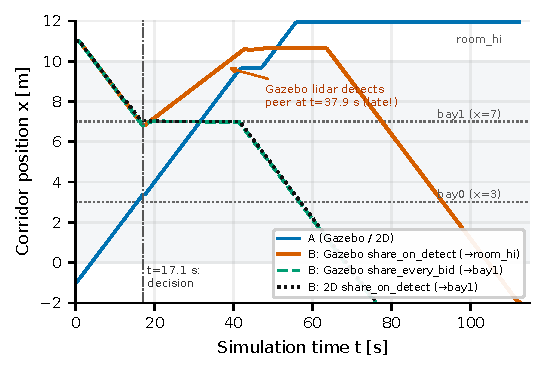
\includegraphics[width=\columnwidth]{Images/fig16_lidar_lag_trace.pdf}
\caption{Empirical spacetime trajectory $x(t)$ on Seed~3 ($R_{\mathrm{det}}=3.5$\,m): wall-filtered Gazebo Lidar clustering lags until $t=37.9$\,s, missing the $t=17.1$\,s decision window and sending $B$ to \texttt{room\_hi} instead of \texttt{bay1}.}
\label{fig:rq4_gz_trace}
\end{figure}

\subsection{Per-condition agreement and delay}
Table~\ref{tab:gzcond} lists every Gazebo condition (460 main runs on the final code plus 36 hold runs) with its paired 2D run; Fig.~\ref{fig:ba} shows the Bland--Altman plot of raw delays. The T-junction rows dominate the limits of agreement.

{\footnotesize
\begin{longtable}{@{}llrrrrl@{}}
\caption{Gazebo versus 2D by condition and policy. Agree: same first yielder. $\Delta D$: Gazebo minus 2D delay over runs successful in both, mean [95\% CI].}\label{tab:gzcond}\\
\toprule group & policy & $n$ & Gz succ. & 2D succ. & agree & $\Delta D$ [s] \\\midrule\endfirsthead
\toprule group & policy & $n$ & Gz succ. & 2D succ. & agree & $\Delta D$ [s] \\\midrule\endhead
S1 & clarke & 10 & 10 & 10/10 & -0.31 [-0.37, -0.26] \\
S1 & forced\_A & 10 & 10 & 10/10 & -0.36 [-0.44, -0.27] \\
S1 & forced\_B & 10 & 10 & 10/10 & -0.44 [-0.55, -0.33] \\
S1 & learned & 10 & 10 & 10/10 & -0.40 [-0.51, -0.29] \\
S1 & reservation & 10 & 10 & 10/10 & -0.35 [-0.36, -0.35] \\
S2\_slow & cost\_bid & 6 & 6 & 6/6 & -0.03 [-0.46, +0.47] \\
S2\_slow & fixed\_priority & 6 & 6 & 6/6 & -0.70 [-0.80, -0.59] \\
S2\_slow & forced\_A & 6 & 6 & 6/6 & +0.40 [-0.16, +0.94] \\
S2\_slow & forced\_B & 6 & 6 & 6/6 & -0.56 [-0.67, -0.42] \\
S2\_slow & rules\_default & 6 & 6 & 6/6 & -0.56 [-0.71, -0.43] \\
S2\_urgent & cost\_bid & 6 & 6 & 6/6 & -0.47 [-0.85, -0.14] \\
S2\_urgent & fixed\_priority & 6 & 6 & 6/6 & -1.43 [-1.73, -1.16] \\
S2\_urgent & forced\_A & 6 & 6 & 6/6 & -0.39 [-0.58, -0.25] \\
S2\_urgent & forced\_B & 6 & 6 & 6/6 & -1.50 [-1.72, -1.29] \\
S2\_urgent & rules\_default & 6 & 6 & 6/6 & -0.41 [-0.67, -0.16] \\
S4 & cost\_bid & 6 & 6 & 6/6 & -0.21 [-0.25, -0.16] \\
S4 & fixed\_priority & 6 & 6 & 6/6 & -0.16 [-0.22, -0.09] \\
S4 & rules\_default & 6 & 6 & 6/6 & -0.17 [-0.26, -0.09] \\
S4\_same\_side & cost\_bid & 4 & 4 & 4/4 & -0.18 [-0.30, -0.07] \\
S4\_same\_side & fixed\_priority & 4 & 4 & 4/4 & -0.12 [-0.15, -0.10] \\
S4\_same\_side & rules\_default & 4 & 4 & 4/4 & -0.26 [-0.37, -0.15] \\
S7 & cost\_bid\_sigma0.5 & 6 & 6 & 4/6 & +1.28 [-1.33, +5.57] \\
S7 & cost\_bid\_sigma1.0 & 6 & 6 & 3/6 & +3.17 [-0.97, +7.43] \\
S8b & cost\_bid & 6 & 6 & 4/6 & -2.95 [-39.27, +26.84] \\
S8b & fixed\_priority & 6 & 6 & 5/6 & +8.89 [-1.05, +26.32] \\
S8c\_all\_off & cost\_bid & 6 & 6 & 5/6 & +11.28 [-0.19, +28.34] \\
S8c\_all\_off & fixed\_priority & 6 & 6 & 4/6 & +2.15 [-15.02, +24.09] \\
S9 & clarke\_ABx0.5 & 6 & 6 & 6/6 & -0.39 [-0.55, -0.27] \\
S9 & clarke\_Ax0.5 & 6 & 6 & 6/6 & -0.36 [-0.53, -0.24] \\
S9 & clarke\_Bx0.5 & 6 & 6 & 6/6 & -0.30 [-0.36, -0.25] \\
asym\_own & cost\_bid & 6 & 6 & 6/6 & -0.39 [-0.42, -0.36] \\
asym\_own & fixed\_priority & 6 & 6 & 6/6 & -0.46 [-0.50, -0.41] \\
asym\_share & cost\_bid & 6 & 6 & 6/6 & -0.22 [-0.24, -0.18] \\
asym\_share & fixed\_priority & 6 & 6 & 6/6 & -0.22 [-0.28, -0.17] \\
comms & cost\_bid & 6 & 6 & 6/6 & -0.49 [-1.52, +0.37] \\
comms & fixed\_priority & 6 & 6 & 6/6 & -0.49 [-1.80, +0.79] \\
comms & rules\_default & 6 & 6 & 6/6 & -0.50 [-1.77, +0.77] \\
convoy & cost\_bid & 6 & 6 & 6/6 & -0.23 [-0.27, -0.19] \\
convoy & fixed\_priority & 6 & 6 & 6/6 & -0.24 [-0.27, -0.21] \\
convoy & group\_bid & 6 & 6 & 6/6 & -0.28 [-0.34, -0.23] \\
convoy & rules\_default & 6 & 6 & 6/6 & -0.23 [-0.27, -0.19] \\
convoy\_B\_urgent & fixed\_priority & 6 & 6 & 6/6 & -1.17 [-1.30, -1.03] \\
convoy\_B\_urgent & group\_bid & 6 & 6 & 6/6 & -1.13 [-1.17, -1.07] \\
corridor & cost\_bid & 10 & 10 & 10/10 & -0.27 [-0.33, -0.21] \\
corridor & fixed\_priority & 10 & 10 & 10/10 & -0.35 [-0.43, -0.27] \\
corridor & reactive & 10 & 6 & 3/10 & -6.62 [-65.22, +39.98] \\
corridor & rules\_default & 10 & 10 & 10/10 & -0.36 [-0.44, -0.28] \\
corridor & rules\_proximity & 10 & 10 & 10/10 & -0.35 [-0.44, -0.27] \\
explore\_all\_3.5 & cost\_bid & 6 & 6 & 6/6 & -0.16 [-0.25, -0.07] \\
explore\_all\_3.5 & fixed\_priority & 6 & 6 & 6/6 & -0.18 [-0.22, -0.14] \\
explore\_all\_6.0 & cost\_bid & 6 & 6 & 6/6 & -0.20 [-0.26, -0.12] \\
explore\_all\_6.0 & fixed\_priority & 6 & 6 & 6/6 & -0.15 [-0.20, -0.11] \\
explore\_det\_3.5 & cost\_bid & 6 & 6 & 5/6 & +0.08 [-0.19, +0.51] \\
explore\_det\_3.5 & fixed\_priority & 6 & 6 & 6/6 & +6.79 [-0.19, +20.68] \\
explore\_det\_6.0 & cost\_bid & 6 & 6 & 6/6 & -0.31 [-0.40, -0.23] \\
explore\_det\_6.0 & fixed\_priority & 6 & 6 & 6/6 & -0.45 [-0.50, -0.41] \\
explore\_full\_3.5 & cost\_bid & 6 & 6 & 6/6 & -0.24 [-0.27, -0.21] \\
explore\_full\_3.5 & fixed\_priority & 6 & 6 & 6/6 & -0.21 [-0.27, -0.15] \\
explore\_none\_3.5 & cost\_bid & 6 & 6 & 6/6 & -0.24 [-0.32, -0.17] \\
explore\_none\_3.5 & fixed\_priority & 6 & 6 & 6/6 & -0.66 [-1.31, -0.27] \\
explore\_none\_6.0 & cost\_bid & 6 & 6 & 6/6 & -0.37 [-0.41, -0.32] \\
explore\_none\_6.0 & fixed\_priority & 6 & 6 & 6/6 & -0.41 [-0.46, -0.38] \\
tj & cost\_bid & 6 & 6 & 6/6 & -44.15 [-86.50, -22.81] \\
tj & fixed\_priority & 6 & 6 & 6/6 & +2.97 [+0.65, +5.18] \\
tj & rules\_default & 6 & 6 & 6/6 & -1.76 [-11.07, +4.17] \\
tjgoal & cost\_bid & 6 & 6 & 6/6 & -11.13 [-11.38, -10.92] \\
tjgoal & fixed\_priority & 6 & 6 & 6/6 & -23.02 [-27.50, -17.32] \\
tjgoal & rules\_default & 6 & 6 & 6/6 & -23.41 [-27.49, -18.09] \\
wrong\_map & cost\_bid & 6 & 6 & 6/6 & -1.14 [-1.26, -1.05] \\
wrong\_map & fixed\_priority & 6 & 6 & 6/6 & -1.21 [-1.31, -1.11] \\
wrong\_map & rules\_default & 6 & 6 & 6/6 & -1.26 [-1.36, -1.14] \\
\bottomrule
\end{longtable}}

\begin{figure}[!ht]\centering
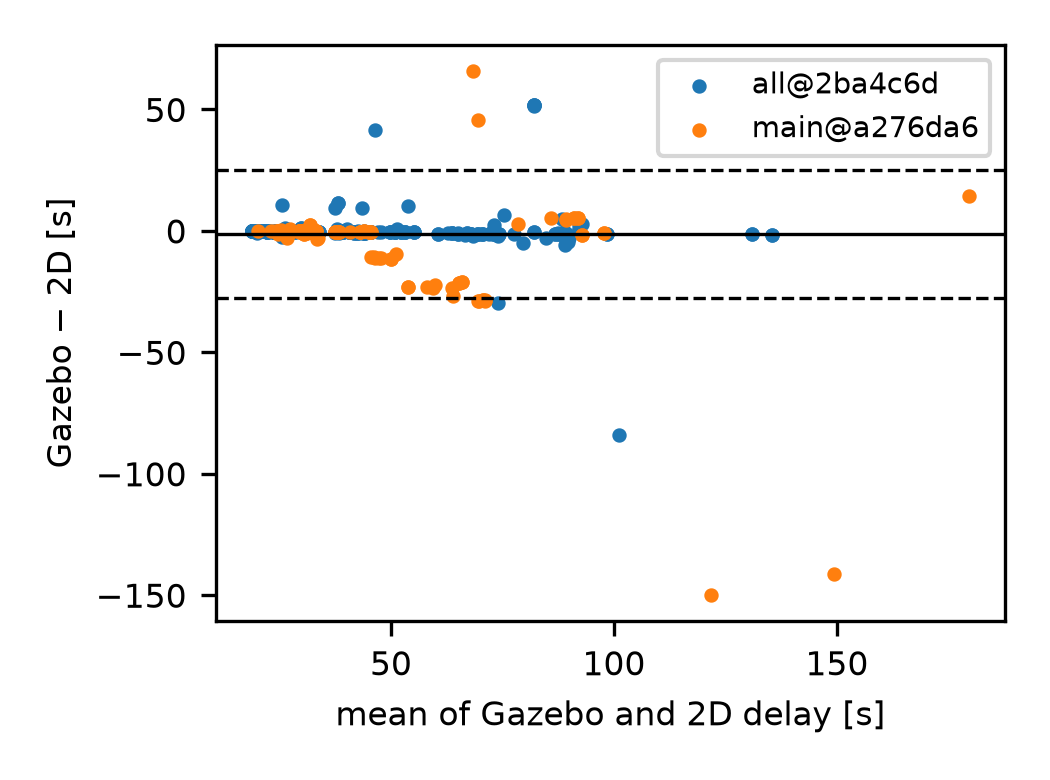
\includegraphics[width=0.6\columnwidth]{Images/gazebo_bland_altman.png}
\caption{Bland--Altman plot of Gazebo versus 2D delay over the 456 runs successful in both simulators: bias $-1.35$\,s, 95\% limits of agreement $-27.6$ to $+24.9$\,s.}
\label{fig:ba}
\end{figure}

\section{Statistics and Reproducibility}
All 2D studies ran on commit \texttt{dfc3d92} (\texttt{studies/run\_all\_2d.sh}, which refuses to run on a modified tree and writes \texttt{studies/results\_raw/COMMIT}). The revision studies add one script each on top of that commit, recorded in \texttt{COMMIT\_wp3}--\texttt{COMMIT\_wp7}. The Gazebo data combine 338 runs of the final release (\texttt{all@2ba4c6d}, amd64 image) and the 122 original cases rerun on the final code (\texttt{main@a276da6}, ARM64 image built from \texttt{ros:jazzy}); \texttt{studies/compare\_gazebo\_rerun.py} compares the rerun with the superseded runs. \texttt{studies/report/tase\_numbers.csv} maps every number in the paper to its source file and row.

\begin{table}[!ht]\centering
\caption{Reproduction commands. All paths are relative to \texttt{amr\_negotiation/}.}
{\footnotesize
\resizebox{\columnwidth}{!}{\begin{tabular}{@{}lll@{}}\toprule
Results & Command & Output \\\midrule
S1--S10, convoy, T-junction, maps, classifier & \texttt{studies/run\_all\_2d.sh} & \texttt{studies/results\_raw/*.csv.gz} \\
Statistics (Tables IV, VI; Holm, TOST) & \texttt{python studies/analyse\_tase.py} & \texttt{studies/report/tase\_stats.md} \\
\texttt{S7d}, \texttt{S7h}, \texttt{S7m} & \texttt{python studies/sigma\_robustness.py}; \texttt{analyse\_sigma.py} & \texttt{report\_r2/sigma\_robustness.md} \\
\texttt{S10b} fairness & \texttt{python studies/fairness\_credit.py} & \texttt{report\_r2/fairness\_credit.md} \\
\texttt{S9b} private types & \texttt{python studies/clarke\_private.py} & \texttt{report\_r2/clarke\_private.md} \\
\texttt{S11a}, \texttt{S11b} baselines & \texttt{python studies/baselines\_r3.py} & \texttt{report\_r2/baselines\_r3.md} \\
\texttt{S8d} correlated loss & \texttt{python studies/burst\_loss.py} & \texttt{report\_r2/burst\_loss.md} \\
Gazebo runs & \texttt{studies/gazebo/run\_case.sh} (jobs in \texttt{runs.txt}, \texttt{runs\_r2.txt}) & \texttt{results\_raw/gazebo\_tase.jsonl.gz} \\
Gazebo analysis (Table~V, S-IV) & \texttt{python studies/analyse\_gazebo\_tase.py} & \texttt{report\_r2/gazebo\_tase.md} \\\bottomrule
\end{tabular}}}
\end{table}

\section{Protocol Architecture}
\begin{figure}[!ht]\centering
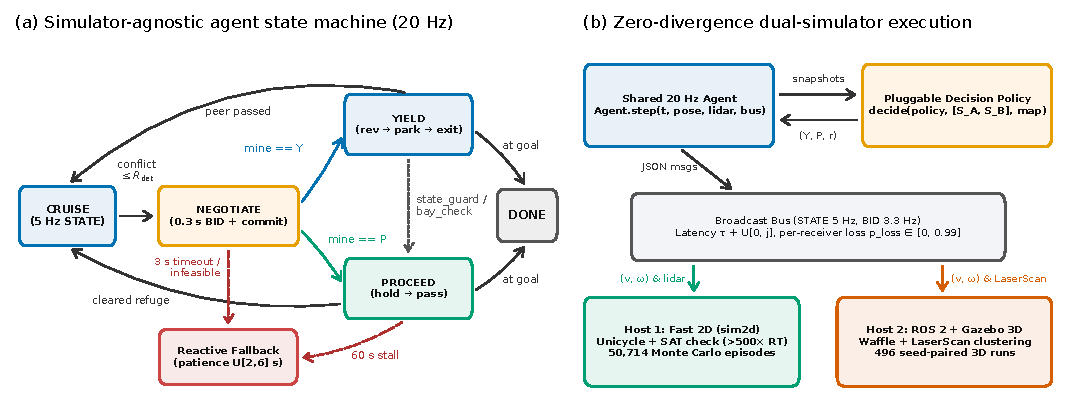
\includegraphics[width=1\textwidth]{Images/protocol.pdf}
\caption{Decentralized negotiation protocol and dual-simulator execution architecture. (a) Simulator-agnostic $20$\,Hz agent state machine showing nominal transitions (solid), timeout/infeasibility reactive fallbacks (dashed red), and lossy-channel yield-abort guards (dotted gray). (b) Zero-code-divergence execution architecture connecting the shared $20$\,Hz \texttt{Agent} controller and pluggable decision policy to both the fast 2D unicycle simulator (\texttt{sim2d}) and 3D ROS~2 Jazzy / Gazebo Harmonic.}
\label{fig:proto}
\end{figure}

\section{Additional Figures}
\begin{figure}[!ht]\centering
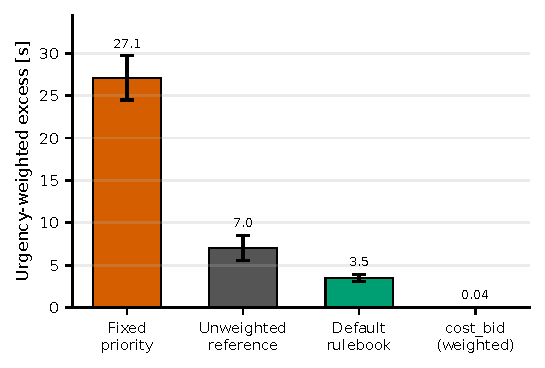
\includegraphics[width=\columnwidth]{Images/fig6_asymmetry.pdf}
\caption{Urgency-weighted excess delay across heterogeneous robot urgency, payload, and speed regimes (\texttt{S2}, $N=5{,}040$). Error bars show 95\% CIs.}
\label{fig:rq1_asym}
\end{figure}

\begin{figure}[!ht]\centering
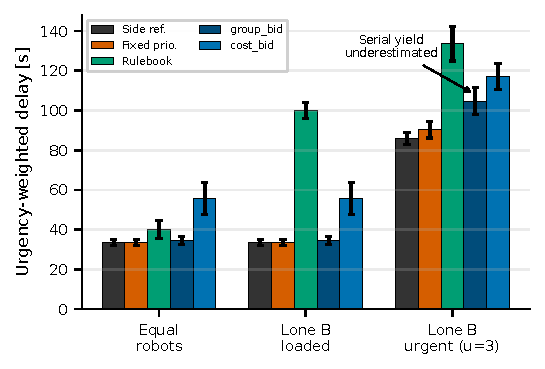
\includegraphics[width=\columnwidth]{Images/fig13_convoy_delay.pdf}
\caption{Convoy 2-vs.-1 urgency-weighted delay ($N=1{,}080$) across equal, loaded-$B$, and urgent-$B$ ($u_B=3$) regimes with follower \texttt{make\_room}. Error bars show 95\% CIs.}
\label{fig:rq4_convoy}
\end{figure}

\bibliographystyle{IEEEtran}
\bibliography{references}
\end{document}
